%%%%%%%%%%%%%%%%%%%%%
%                                             %
%                 Experiment M-3              %
%               g with a pendulum             %
%                                             %
%%%%%%%%%%%%%%%%%%%%%

% Hyperref doesn't like math in chapter titles.
\iffalse
\labChapter{M}{Simple Projectile Motion with Kinematics}
\else
\labChapter{M}{Simple Projectile Motion with Kinematics}
\fi
\label{lab:M3}






% Background
\section{Background}


\textbf{Projectile motion} is the motion of an object thrown or projected into the air, subject only to acceleration as a result of gravity. The applications of projectile motion in physics and engineering are numerous. Some examples include meteors as they enter Earth’s atmosphere, water in a water fountain, and the motion of any ball in sports. Such objects are called \textit{projectiles}, and their path is called a \textbf{trajectory}. 

We can represent a projectile's motion through kinematics which utilize its position, time, velocity, and acceleration. The kinematic equations we will use during this lab assume both \textbf{\textit{constant acceleration}} effects of air resistance are \textbf{\textit{negligible}} (generalized in the next four equations with $x$ representing position along any given dimension):

 \begin{equation}
  \label{eq:M03Kinematic_01}
  v = v_{0} + at
\end{equation}


 \begin{equation}
  \label{eq:M03Kinematic_02}
  x = x_{0} + v_{0}t + \frac{1}{2}at^{2}
\end{equation}


 \begin{equation}
  \label{eq:M03Kinematic_03}
  v^{2} = v_{0}^{2} + 2a(x - x_{0})
\end{equation}

 \begin{equation}
  \label{eq:M03Kinematic_04}
  x = x_{0} + \frac{1}{2}(v_{0} + v)t
\end{equation}



\pagebreak


Today, we will analyze both one- and two-dimensional trajectories, where $x$ will represent the horizontal direction, and $y$ the vertical. Gravity (which pulls objects down towards the center of the Earth) will be assumed to be the only source of acceleration acting on our projectiles; as such, the acceleration of a projectile is $a_{y} = -g$ and $a_{x} = 0$. Since horizontal acceleration terms are zero, we can represent horizontal motion by:

 \begin{equation}
  \label{eq:M03horizontalKinematic}
  v_{0x} = v_{x} = \text{constant velocity},~~~ x = x_{0} + v_{x}t
\end{equation}

Then, depending on the information we have available to us, we can represent vertical motion by:

 \begin{equation}
  \label{eq:M03Kinematic_vertical_01}
  v_{y} = v_{0y} - gt
\end{equation}


 \begin{equation}
  \label{eq:M03Kinematic_vertical_02}
  y = y_{0} + v_{0y}t - \frac{1}{2}gt^{2}
\end{equation}


 \begin{equation}
  \label{eq:M03Kinematic_vertical_03}
  v_{y}^{2} = v_{0y}^{2} - 2g(y - y_{0})
\end{equation}

 \begin{equation}
  \label{eq:M03Kinematic_vertical_04}
  y = y_{0} + \frac{1}{2}(v_{0y} + v_{y})t
\end{equation}







\underline{\textbf{Free Fall / Downward Trajectory (First experiment)}}

In the previous lab, we determined the acceleration due to gravity via the tilted air track to take advantage of a longer time frame to measure a small fraction of the acceleration due to gravity. This week, we will determine the acceleration due to gravity more directly by considering a one-dimensional trajectory (i.e. free fall).



The experimental setup will involve a free-fall timer where a metal ball is dropped from a release mechanism as shown in Fig.~\ref{M03_simpleProjectileLauncher_Exp1}. When the metal ball is in then mechanism, it provides a closed circuit; once the ball is released and the circuit opens, the computer automatically starts timing $t_{\text{initial}}$. The ball then hits the receptor pad on the floor, closing the circuit and stopping the timer at $t_{\text{final}}$. Using the recorded time difference $t = t_{\text{final}} - t_{\text{initial}}$, and the initial height $y_{0}$ as measured from the bottom of the ball to the top of the receptor plate (which is at the final height $y = 0\,\meter$), we can rearrange Eqn.~\ref{eq:M03Kinematic_vertical_02} to determine acceleration due to gravity.

 \begin{equation}
  \label{eq:M03Kinematic_freefall_g}
  0 = y_{0} + 0 - \frac{1}{2}gt^{2}~~~=>~~~\frac{2y_{0}}{t^2} = g
\end{equation}

\begin{figure}[h]
  \begin{center}
    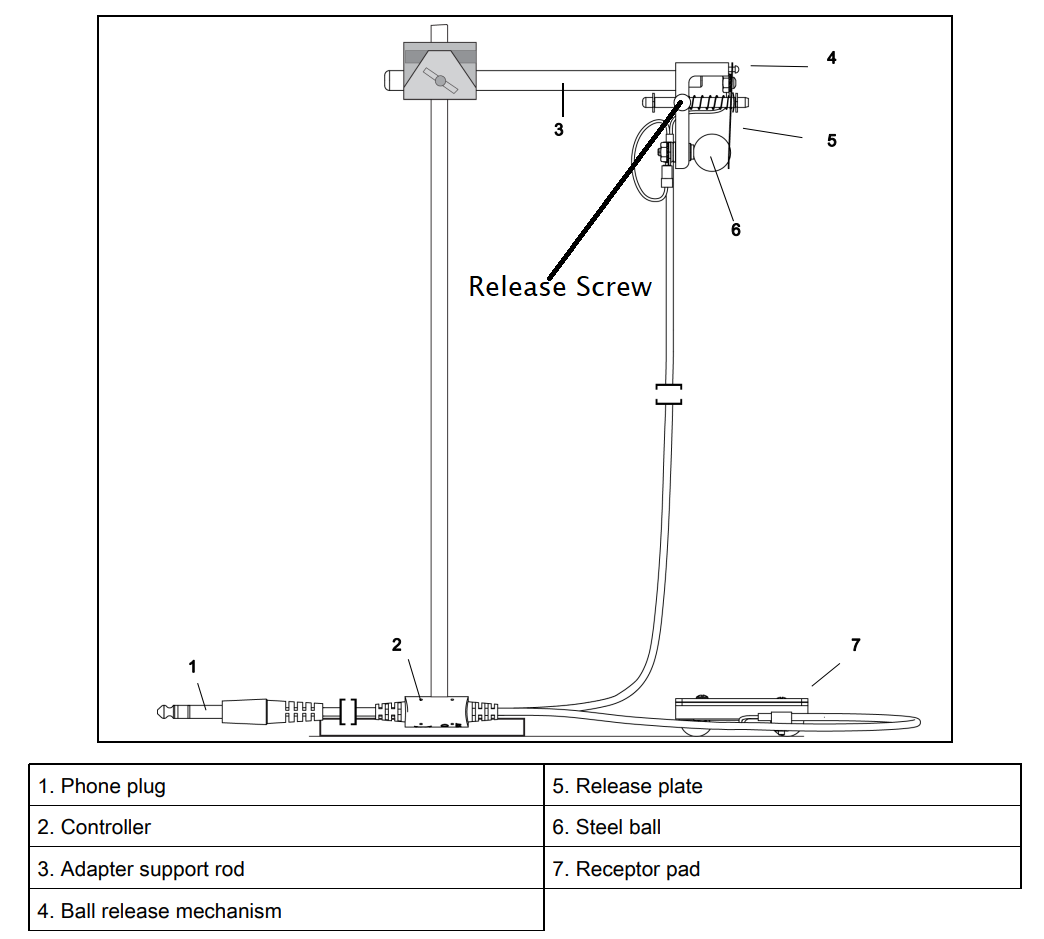
\includegraphics[width=4.9in]{Fall/Experiment03FiguresNEW/M3_Exp1.png}
  \end{center}
  \caption{Example of the free fall apparatus used in Exp. 1. Note the release screw will be what you tighten or loosen to hold or release the ball from the release mechanism.}
  \label{M03_simpleProjectileLauncher_Exp1}
\end{figure}

\pagebreak

\underline{\textbf{Horizontal Trajectory (Second experiment)}}


\begin{figure}[h]
  \begin{center}
    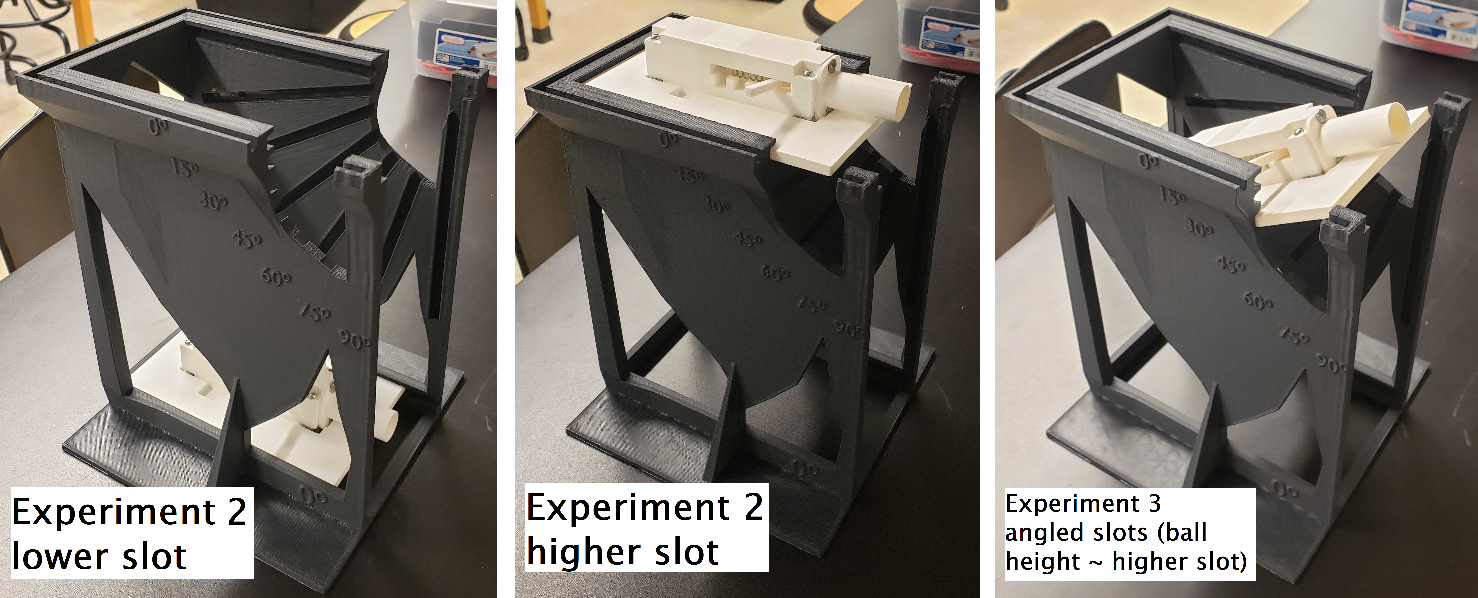
\includegraphics[width=5.9in]{Fall/Experiment03FiguresNEW/M3_ExpOptions_quarter_size.png}
  \end{center}
  \caption{Left) Position of launcher for lower height in Experiment 2. Right) Position of launcher for higher height in Experiment 2. Right) Position of launcher for angled launches in Experiment 3 where the ball's initial position is the same as the higher height position.}
  \label{M03_simpleProjectileLauncher}
\end{figure}


Note: For this experiment as well as the third experiment later on, while we could use our determined value for gravity, for simplicity, we will instead use the accepted value of $g = 9.803\,\meter\per\second\squared$ for Fairfield, CT.

In this second experiment, we will \textbf{1)} first investigate the horizontally launched trajectory of the same metal ball used in the first experiment (launched at 90$\degree$ relative to $g$, or 0$\degree$ relative to the floor). Then \textbf{2)} we will attempt to estimate where the ball will land when launched from a different height and see how accurate we are.

This setup will involve a marble launcher that can slide into a large holder at different initial heights $y_{0}$ (and later for the third experiment, different angles, see Fig.~\ref{M03_simpleProjectileLauncher}). Height $y_{0}$ will be measured from the bottom of the ball (effectively the bottom inside of the launcher's barrel) to the floor. Once the ball is released, it will begin a two-dimensional trajectory accelerated solely by gravity in the $y$ direction.

\underline{\textbf{-1-)}} The distance in the $x$ direction will be measured from the center of the ball in the uncocked position (a plum bob can be used to find the ball's initial position on the floor) to the average landing position on the floor after the given number of trials. The ball will mark up paper with carbon paper; we will circle this scatter shot and estimate the average position of all trials from the given case, and then measure the distance with a 1 or 2 meter stick to determine $x$.

After investigating how far the ball travels in the $x$ direction from a given height, we can determine characteristics about the launcher-and-ball system to estimate how far in the $x$ direction we may expect the ball to travel in the second part of this experiment when we launch it from a different initial height. To estimate how far the ball will travel, we can use Eqn.~\ref{eq:M03horizontalKinematic} to determine $x$. However, to do so, we will need to for how long and how fast it was moving (distance traveled = speed $\times$ time). Since we know the initial height $y_{0}$ of the ball, we can determine the time $t$ it took to fall to the floor in the $y$ direction due solely to gravity $g$ by rearranging Eqn.~\ref{eq:M03Kinematic_vertical_02} to solve for $t$, knowing that $v_{0y} = 0\,\meter\per\second$ and treating the floor as $y = 0\,\meter$:

 \begin{equation}
  \label{eq:M03Kinematic_vertical_time}
  0 = y_{0} + 0 - \frac{1}{2}gt^{2}~~~=>~~~\sqrt{\frac{2y_{0}}{g}} = t
\end{equation}

Now that we know the time $t$ of the trajectory, and treating the uncocked position as $x_{0} = 0\,\meter$, we can use Eqn.~\ref{eq:M03horizontalKinematic} to determine the horizontal velocity $v_{x}$ when released:

 \begin{equation}
  \label{eq:M03Kinematic_horizontal_velocity_01}
  x = 0 + v_{x}t~~~=>~~~\frac{x}{t} = v_{x}
\end{equation}

\underline{\textbf{-2-)}} For the second part of this experiment, we move the launcher to the higher $0\degree$ slot ($\sim20\,\centi\meter$ higher), and we want to determine how far it will travel in the $x$ direction. This leads us back to Eqn.~\ref{eq:M03horizontalKinematic} where we want to solve for $x_{\text{higher height}}$ (where again, $x_{0} = 0\,\meter$ in the uncocked position):

 \begin{equation}
  \label{eq:M03Kinematic_horizontal_velocity_02}
  x = 0 + v_{x}t~~~=>~~~x_{\text{higher height}} = v_{x}t_{\text{higher height}}
\end{equation}

We know the ball's velocity $v_{x}$, but we no longer know the time. However, similar to before, we can solve for $t_{\text{higher height}}$ by plugging $y_{0\text{,higher height}}$ into Eqn.~\ref{eq:M03Kinematic_vertical_time}:

 \begin{equation}
  \label{eq:M03Kinematic_vertical_time_higher_height}
  \sqrt{\frac{2y_{0\text{,higher height}}}{g}} = t_{\text{higher height}}
\end{equation}

This subsequent value for time $t_{\text{higher height}}$ can be used in Eqn.~\ref{eq:M03Kinematic_horizontal_velocity_02} to then calculate a theoretical distance $x_{\text{higher height, theoretical}}$. We will then launch the ball from this higher height see how accurate we estimated $x_{\text{higher height, theoretical}}$. The experimentally determined $x_{\text{higher height, experimental}}$ will be measured in the same way as the first part of this experiment (circling and estimating the center of the scattershot).



\underline{\textbf{Angled Trajectory (Third experiment)}}




The third part of this experiment is similar to the 2nd part of the second experiment in that we are staying at the higher height, but now investigating the trajectories when launched from different angles, namely, how far in the $x$ direction do they reach? The large, launcher holder is designed to hold the ball at rest (uncocked) in the same position (height) regardless of angle, so you should be able to use your previously determined $y_{0\text{,higher height}}$ as your value for the ball's initial height (see Fig.~\ref{M03_simpleProjectileLauncher} right).

By launching at an upward angle $\theta$, we are now giving some of the initial velocity to both $x$ and $y$ directions. Once again, as there is no acceleration in the $x$ direction, we will ultimately use Eqn.~\ref{eq:M03horizontalKinematic} to determine $x_{\theta}$. However, we need to know both $v_{x\theta}$ and $t_{\theta}$. The velocity will merely be the horizontal component of the launch angle:


 \begin{equation}
  \label{eq:M03Kinematic_horizontal_velocity_03}
    v_{x\theta} = v_{x}\cos{\theta} 
\end{equation}

\begin{figure}[h]
  \begin{center}
    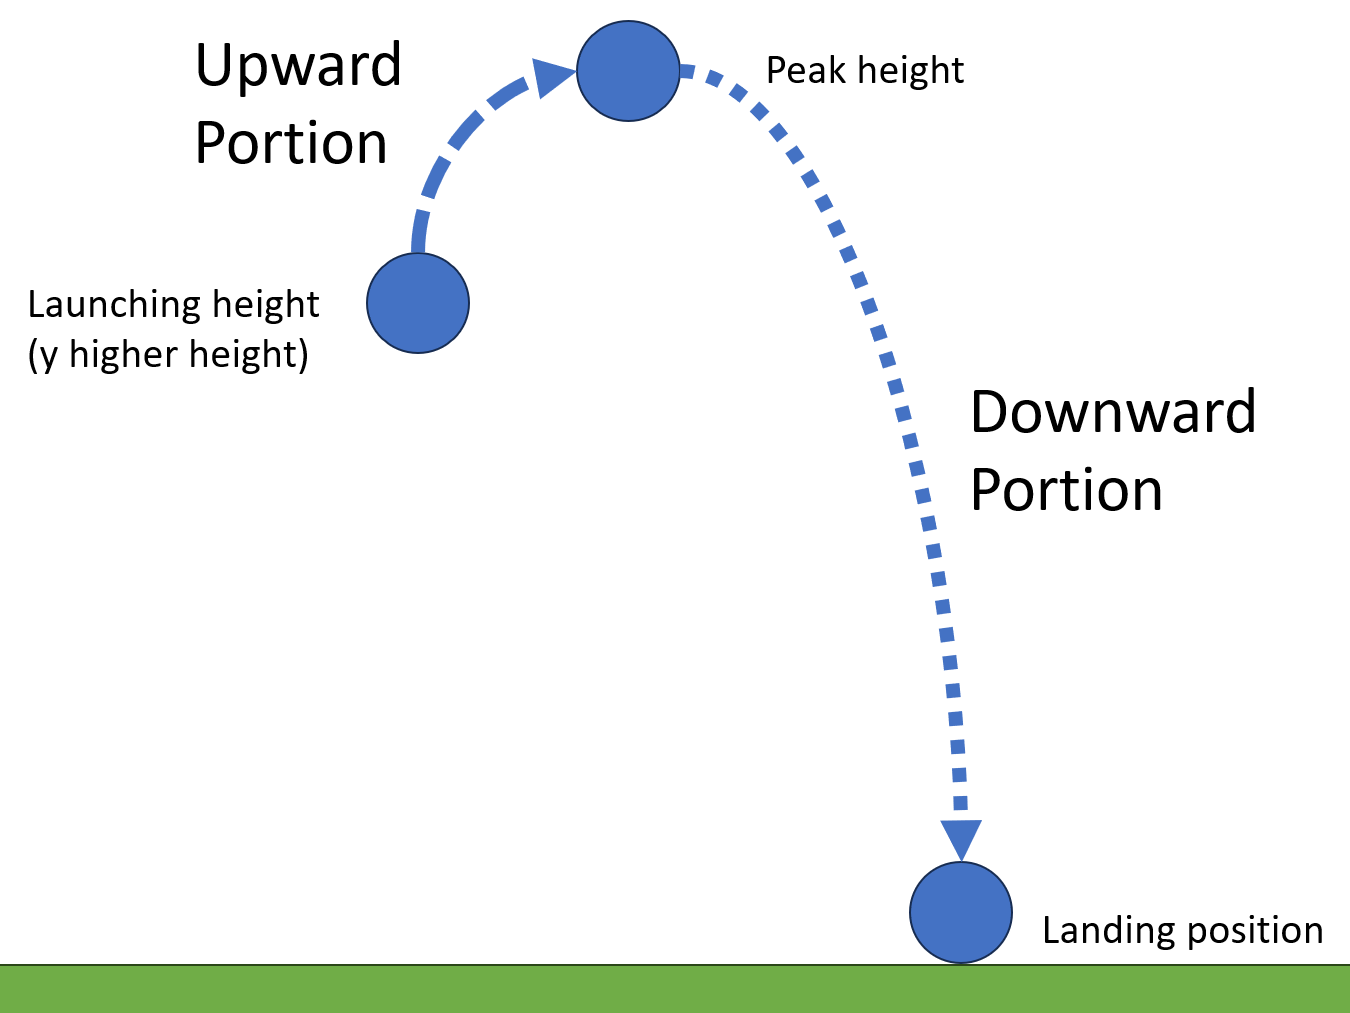
\includegraphics[width=3.9in]{Fall/Experiment03FiguresNEW/M3_Exp3.png}
  \end{center}
  \caption{Example of the upward and downward portions you'll analyze in Experiment 3 for an angled launch.}
  \label{M03_simpleProjectileLauncher_Exp3}
\end{figure}

To solve for the time, however, we can characterize motion in the $y$ direction to determine for how long the ball is in the air.
%Using the same process as before where the floor is at $y_{0} = 0\,\meter$, and $v_{0y} = v_{x}\sin{\theta}$, we can find $t_{\theta}$ 
%using Eqn.~\ref{eq:M03Kinematic_vertical_02} and the quadratic formula:
%
%
% \begin{equation}
%  \label{eq:M03Kinematic_vertical_time_03}
%  y = 0 + v_{0y}t - \frac{1}{2}gt^{2}~~~=>~~~y = 0 + v_{x}\sin{\theta}t_{\theta} - \frac{1}{2}gt_{\theta}^{2}~~~=>
%\end{equation}
%
%
% \begin{equation}
%  \label{eq:M03Kinematic_vertical_time_03_pt2}
% =>~~~\frac{1}{2}gt_{\theta}^{2} - v_{x}\sin{\theta}t_{\theta} + y = 0~~~=>~~~t_{\theta} = \frac{-(-v_{x}\sin{\theta}) \pm \sqrt{((-v_{x}\sin{\theta})^2 - 4\frac{g}{2}y)}}{2\frac{g}{2}}
%\end{equation}
%
% \begin{equation}
%  \label{eq:M03Kinematic_vertical_time_03_pt3}
% =>~~~t_{\theta} = \frac{v_{x}\sin{\theta} \pm \sqrt{((-v_{x}\sin{\theta})^2 - 2gy)}}{g}
%\end{equation}
%
%Note: we would take the larger value as we are launching the ball upwards rather than the smaller value that would represent shooting down towards the floor.
%
As shown in Fig.~\ref{M03_simpleProjectileLauncher_Exp3}, we can find that total time by breaking the trajectory into parts (i.e. $t_{\theta}~=~t_{\text{up}}~+~t_{\text{down}}$) where $t_{\text{up}}$ is the time for upward travel to the peak height, and $t_{\text{down}}$ is the time for downward travel to the floor from that peak height. \textbf{UPWARD PORTION)} Starting with Eqn.~\ref{eq:M03Kinematic_vertical_01}, where we know for the upward travel portion the initial velocity in the $y$ direction is $v_{0y} = v_{0y\text{ higher height}} = v_{x}\sin{\theta}$ and at the peak of the trajectory (end of the upward travel) $v_{y} = v_{y\text{peak}} = 0\,\meter\per\second$, thus:

 \begin{equation}
  \label{eq:M03Kinematic_vertical_time_03_v2_pt1}
  v_{y\text{ peak}} = v_{0y\text{ higher height}} - gt~~~=>~~~0 = v_{x}\sin{\theta} - gt_{\text{up}}~~~=>~~~\frac{v_{x}\sin{\theta}}{g} = t_{\text{up}}
\end{equation}

\textbf{DOWNWARD PORTION)} Then for the downward travel, we need to first know how high we travelled during the upward portion (i.e. $y_{0\text{,higher height}} \text{ to } y_{\text{ peak}}$) so we can use Eqn.~\ref{eq:M03Kinematic_vertical_02} later to determine the time it took to fall from $y_{\text{ peak}} \text{ to } y_{\text{ floor}}$. Since we know our initial height $y_{0} = y_{0\text{,higher height}}$, initial velocity $v_{0} = v_{0y\text{ higher height}} = v_{x}\sin{\theta}$, and the time it took to get $t_{\text{up}}$ there from Eqn.~\ref{eq:M03Kinematic_vertical_time_03_v2_pt1}, we can use Eqn.~\ref{eq:M03Kinematic_vertical_02} to solve for the final height of the upward travel $y_{\text{peak}}$:

 \begin{equation}
  \label{eq:M03Kinematic_vertical_time_03_v2_pt2}
  y_{\text{peak}} = y_{0\text{,higher height}} + v_{x}\sin{\theta}t_{\text{up}} - \frac{1}{2}gt_{\text{up}}^{2}
\end{equation}


Now that we know $y_{\text{peak}}$, we can use Eqn.~\ref{eq:M03Kinematic_vertical_02} to solve for $t_{down}$, this time with the final height $y_{\text{floor}} = 0\,\meter$, initial height of $y_{\text{peak}}$, and the initial velocity $v_{y\text{ peak}} = 0\,\meter\per\second$.


 \begin{equation}
  \label{eq:M03Kinematic_vertical_time_03_v2_pt3}
  y_{\text{floor}} = y_{\text{peak}} + v_{y\text{ peak}} - \frac{1}{2}gt_{\text{down}}^{2}~~~=>~~~0 = y_{\text{peak}} + 0 - \frac{1}{2}gt_{\text{down}}^{2}~~~=>~~~\sqrt{\frac{2y_{\text{peak}}}{g}} = t_{\text{down}}
\end{equation}


\textbf{HORIZONTAL DISTANCE)} Finally, we have the total time $t_{\theta}~=~t_{\text{up}}~+~t_{\text{down}}$ from Eqns.~\ref{eq:M03Kinematic_vertical_time_03_v2_pt1} and ~\ref{eq:M03Kinematic_vertical_time_03_v2_pt3} and the initial velocity $v_{x}$ from Eqn.~\ref{eq:M03Kinematic_horizontal_velocity_03} to incorporate into Eqn.~\ref{eq:M03horizontalKinematic} to determine the theoretical distance $x_{\theta}$ the ball with travel in the $x$ direction for any given angle $\theta$:

 \begin{equation}
  \label{eq:M03Kinematic_vertical_time_03_v2_pt4}
  x_{\theta} = v_{x}\cos{\theta}t_{\theta}
\end{equation}



%Experimental Procedure
\section{Experimental Procedure}


\subsection{EXPERIMENT 1 -- Free Fall / Downward Trajectory}


%\TEXTBF{FIRST EXPERIMENT} We study one-dimensional trajectory (free fall)


\begin{enumerate}
\item \textbf{OVERALL GOALS:} 
\begin{itemize}
    \item Investigate projectile motion in one-dimension ($y$).
    \item Conduct 5 trials of the free-fall and determine acceleration due to gravity using one-dimensional kinematics.
    \item \textit{POINT TO CONSIDER}: Will this experiment be more or less accurate in measuring $g$ than the previous lab using gliders on a tilted air track?
    \item \textit{NOTE}: There are only 4 setups, please share, and once you're done taking your data, move on to ensure other groups have a reasonable chance to use the apparatus.
    %\textit{TO CONSIDER}: On the moon, would the ball fall faster, slower, or the same speed as ?
    \item PASCO TIMER Precision: 0.0001 seconds
\end{itemize}


\item Create a data table for this experiment:
\begin{itemize}
    \item Common data section with the accepted value of $g$, the ball height $y_{0}$, and the ball height's estimated uncertainty $\delta y$.
    \item With \textbf{five rows} (1 for each of the 5 free-fall trials). Also include additional \textbf{rows} for the average $g$ value, the $\pm$ uncertainty in gravity $\delta g$, the magnitude difference compared to the accepted $g$ \textit{DISCUSSION POINT for later}: How well does you average value of $g \pm \delta g$ agree with the accepted value of $g$?).
    \item Include \textbf{six columns} for
    \begin{itemize}
        \item Initial time $t_{\text{initial}}$
        \item Initial time uncertainty $\delta t_{\text{initial}}$
        \item Final time $t_{\text{final}}$
        \item Final time uncertainty $\delta t_{\text{final}}$
        \item Total elapsed time $t = t_{\text{final}} - t_{\text{initial}}$
        \item Total elapsed time uncertainty $\delta t = t_{\text{final}} - t_{\text{initial}}$
        \item Calculated $g$
    \end{itemize} 
\end{itemize}
\item CAPSTONE will be set up with the Free-Fall Adapter which, whenever the circuit opens or closes, will record the time that event occurred.
\item Place your metal ball from your marble launcher into the spring loaded holder at one of the four setups. You will need to push the metal tab in and then hand-tighten the holding/release screw to hold the ball in place.
\item Ensure the receptor pad is beneath the ball such that it hits close to the open side.
\item Measure the height the ball will fall; the initial height $y_{0}$ is measured from the bottom of the ball to the top of the receptor plate which has a final height $y = 0\,\meter$ if you place the meter stick on the receptor pad.
\item Press Record in CAPSTONE. You can let it run and it'll continue collecting data even when you reset the ball for additional trials; or restart for each trial, just be aware of which data points are related to your drop.
\item Unscrew the holding/release screw to allow the ball to fall.
\item Record your $t_{\text{initial}}$ and $t_{\text{final}}$ times.
\item Repeat the drop for a total of 5 free-fall trials. Determine the total elapsed times $t$ for each trial.
\item Using Eqn.~\ref{eq:M03Kinematic_freefall_g}, calculate the value of $g$ for each of your trials (benefit here of calculating $g$ from each trial: you can more easily notice any outlier data).
\item Determine your average $g$ from the preceding values.
\item Estimate your uncertainty in $g$, as represented by $\delta g = g_\text{test} - g$, (i.e. how confident [$\pm$] you are in what you measured -- e.g. distance, time). Plug in each measurements' uncertainties to make your test value of $g_\text{test}$ as calculated with Eqn.~\ref{eq:M03Kinematic_freefall_g} as big as possible (i.e. larger numerator, smaller denominator). Determine $\delta g$.
\item Compare your average $g$ to the accepted value of $g = 9.803\,\meter\per\second\squared$; what is the total difference?
%\item Compare your average $g$ to the accepted value of $g = 9.803\,\meter\per\second\squared$; what is the \% difference?
\item Does you average $g \pm \delta g$ cover the difference from the accepted value and agree, or not?

\end{enumerate}


\subsection{Horizontal Trajectory (Second experiment)}



\begin{enumerate}
\item \textbf{OVERALL GOALS:} 
\begin{itemize}
    \item Investigate projectile motion in two-dimensions when launched horizontally.
    \item For simplicity and to decrease error propagation, \textbf{for the rest of lab, assume and use} the accepted value of $g = 9.803\,\meter\per\second\squared$ for Fairfield, CT rather than your previously determined value.
    \item Characterize the trajectory from the marble launcher at initial height.
    \item Calculate the theoretical trajectory (distance $x$) for a different height; place a bullseye at your expected location and compare your experimental landing scattershot to the theoretical distance.
    \item Conduct 20 launches for each height; estimate the experimental landing scattershot by circling your carbon-paper dots and estimating the center of the scattershot.
    %\item \textit{POINT TO CONSIDER}: Will this experiment be more or less accurate in measuring $g$ than the previous lab using gliders on a tilted air track?
    %\item \textit{NOTE}: There are only 4 setups, please share, and once you're done taking your data, move on to ensure other groups have a reasonable chance to use the apparatus.
    %\textit{TO CONSIDER}: On the moon, would the ball fall faster, slower, or the same speed as ?
\end{itemize}


\item Create a data table for this experiment:
\begin{itemize}
    \item Common data section with the accepted value of $g$.
    \item Section for the case at a the lower initial height containing:
    \begin{itemize}
        \item the ball height $y_{0}$
        \item the ball height's estimated uncertainty $\delta y_{0}$
        \item distance $x$
        \item distance uncertainty $\delta x$ based on the radius of the circle you draw around the scattershot
    \end{itemize} 
    \item Additional sections for derived time of the trajectory $t$ and velocity $v_{x}$
    \item Additional sections for:
    \begin{itemize}
        \item Height of the ball at the higher $0 \degree$ slot height $y_{0\text{,higher height}}$
        \item Time of the trajectory from a higher height $t_{\text{higher height}}$
        \item Theoretical distance $x_{\text{higher height, theoretical}}$ (calculated with Eqn.~\ref{eq:M03Kinematic_horizontal_velocity_02})
        \item Experimentally measured distance $x_{\text{higher height, experimental}}$
        \item Estimated uncertainty in the experimental distance $\delta x_{\text{higher height, experimental}}$ (essentially $\pm$ the radius of the circle drawn around your scattershot)
        \item Difference (magnitude) between the theoretical and experimental $x$ distances
    \end{itemize}
\end{itemize}
\item Place the marble launcher in the holder in the lower $0\degree$ slot (uncocked to represent where the ball will be once the piston is no longer accelerating the ball up to speed)
\item Measure the height the ball will fall; place the metal ball into the launcher as the initial height $y_{0}$ is measured from the bottom of the ball to the floor (though the bottom of the inside of the barrel can also be used as the bottom of the ball location if that is easier to measure).
\item \label{M03_launchStepStart} Conduct a couple test launches by pulling the piston to the first or second notches (whichever position provides the shorter, $\sim 1\,\meter$, $x$ distance). Take mental note of where the ball is generally landing.
\item Get a piece of paper and tape it in the approximate location, and place (no tape needed) a piece of carbon paper on top (no need to tape that one) so the ball can mark up the paper when it lands.
\item Conduct \textbf{20 launches} onto the paper/carbon paper.
\item Put aside the carbon paper and mark the dots with a marker or something else that makes it apparent which dots are your data points for this height. Draw a rough circle surrounding the scattershot and visually estimate the center by drawing a cross hair to represent the center of the scatter.
\item Measure the experimental distance $x$ from the center of the ball at rest in the barrel (uncocked) to the cross hair center that you drew in your scatter shot on the floor. To translate the initial location of the ball in the barrel to the floor, you can use a plum bob to make a straight line down to the floor, from which you can more easily measure $x$
\item \label{M03_launchStepEnd} From your circle around your scattershot, estimate your uncertainty in distance $\delta x$
\item Move the marble launcher to the higher $0 \degree$ slot and remeasure the initial height $y_{0\text{,higher height}}$
\item Now calculate the theoretical distance $x_{\text{higher height, theoretical}}$ using Eqns.~\ref{eq:M03Kinematic_vertical_time} -- ~\ref{eq:M03Kinematic_vertical_time_higher_height}
\item Repeat steps~\ref{M03_launchStepStart}~to~\ref{M03_launchStepEnd} to determine experimentally the distance with its uncertainty at the higher height (i.e. $x_{\text{higher height, experimental}}$ and $\delta x_{\text{higher height, experimental}}$). \textbf{ADDITIONALLY: Before any launches from the higher height, draw a bullseye at the theoretical distance you expect the balls at the higher height to land to visually see how close we get. You can draw both a cross hair for the distance and estimate how big the scatter will be (to discuss later in Sec.~\ref{M3_InterpretationProjectile}).}
\item Calculate the difference between you theoretical and experimental values of $x$ at the higher height.
\item DISCUSSION POINT (covered in Sec.~\ref{M3_InterpretationProjectile}): Does your experimental distance of the higher height agree with what you expected from your theoretical calculation? In other words, does $x_{\text{higher height, experimental}} \pm \delta x_{\text{higher height, experimental}}$ overlap with $x_{\text{higher height, theoretical}}$ (i.e. does your uncertainty cover the difference between the experimental and theoretical values?)?
\end{enumerate}










\subsection{Angled Trajectory (Third experiment)}



\begin{enumerate}
\item \textbf{OVERALL GOALS:} 
\begin{itemize}
    \item Investigate projectile motion in two-dimensions when launched at a non-zero angle (for now, we'll use the 45\degree slot; if labs go well this semester, we may add additional angles).
    \item Continue to use the accepted value of $g = 9.803\,\meter\per\second\squared$ for Fairfield, CT rather than your previously determined value.
    \item Calculate the theoretical trajectory (distance $x$) for a non-zero angle; place a bullseye at your expected location and compare your experimental landing scattershot to the theoretical distance.
    \item Compare the theoretical trajectory's $x$ distance to the experimentally determined distance.
    \item Conduct 20 launches for each angle; estimate the experimental landing scattershot by circling your carbon-paper dots and estimating the center of the scattershot, with your uncertainty represented by the radius of the drawn circle.
    %\item \textit{POINT TO CONSIDER}: Will this experiment be more or less accurate in measuring $g$ than the previous lab using gliders on a tilted air track?
    %\item \textit{NOTE}: There are only 4 setups, please share, and once you're done taking your data, move on to ensure other groups have a reasonable chance to use the apparatus.
    %\textit{TO CONSIDER}: On the moon, would the ball fall faster, slower, or the same speed as ?
\end{itemize}






\item Create a data table for this experiment:
\begin{itemize}
    \item Common data section with the accepted value of $g$ and any values you will need from previous experiments to determine the theoretical distance at a given angled launch $x_{\theta}$ (Eqns.~\ref{eq:M03Kinematic_horizontal_velocity_03}~to~\ref{eq:M03Kinematic_vertical_time_03_v2_pt4}).
    %\item Section for the case at a the lower initial height containing:
    %\begin{itemize}
    %    \item the ball height $y_{0}$
    %    \item the ball height's estimated uncertainty $\delta y_{0}$
    %    \item distance $x$
    %    \item distance uncertainty $\delta x$ based on the radius of the circle you draw around the scattershot
    %\end{itemize} 
    %\item Additional sections for derived time of the trajectory $t$ and velocity $v_{x}$
    \item Additional sections for:
    \begin{itemize}

    
        %\item Height of the ball at the higher $0 \degree$ slot height $y_{0\text{,higher height}}$ to be carried over from Experiment 2
        %\item Time of the trajectory from a higher height $t_{\text{higher height}}$
        \item Theoretical distance $x_{\theta\text{, theoretical}}$ (calculated with Eqn.~\ref{eq:M03Kinematic_vertical_time_03_v2_pt4})
        \item Experimentally measured distance $x_{\theta\text{, experimental}}$
        \item Estimated uncertainty in the experimental distance $\delta x_{\theta, experimental}$ (essentially $\pm$ the radius of the circle drawn around your scattershot)
        \item Difference (magnitude) between the theoretical and experimental $x$ distances
    \end{itemize}
\end{itemize}

\item Place the marble launcher in the holder in the $45\degree$ slot
\item Use your previously measured $y_{0\text{,higher height}}$ as the height the ball will fall for any angled launches (e.g. $y_{0\text{,higher height}} = y_{\theta\text{,higher height}}$).
%\item Measure the height the ball will fall; place the metal ball into the launcher as the initial height $y_{0}$ is measured from the bottom of the ball to the floor (though the bottom of the inside of the barrel can also be used as the bottom of the ball location if that is easier to measure).
\item \label{M03_launchStepStart_exp3} Calculate the theoretical distance $x_{\text{, theoretical}}$ using Eqns.~\ref{eq:M03Kinematic_horizontal_velocity_03}~to~\ref{eq:M03Kinematic_vertical_time_03_v2_pt4}
\item Before any launches from the higher height, tape a paper and draw a bullseye at the theoretical distance you expect the balls at the given angle to land to visually see how close we get. You can draw both a cross hair for the distance and estimate how big the scatter will be.
\item Conduct a few test launches by pulling the piston to the same notch you've been using in Experiment 2 to be able to use the same exit velocity as previously determined
\item If need be, tape additional paper in the location from the test launches. Place (no tape needed) a piece of carbon paper on top (no need to tape that one) so the ball can mark up the paper when it lands.
\item Conduct \textbf{20 launches} onto the paper/carbon paper.
\item Put aside the carbon paper and mark the dots with a marker or something else that makes it apparent which dots are your data points for this height. Draw a rough circle surrounding the scattershot and visually estimate the center by drawing a cross hair to represent the center of the scatter.
\item Measure the experimental distance $x$ from the center of the ball at rest in the barrel (uncocked) to the cross hair center that you drew in your scatter shot on the floor. The initial position of the ball in the $x$ direction translated to the floor should be the same as Experiment 2 (to save you some time). Remeasure if that's no longer the case (e.g. you've accidentally moved the launcher holder)
\item From your circle around your scattershot, estimate your uncertainty in distance $\delta x$
\item \label{M03_launchStepEnd_exp3}  Calculate the difference between you theoretical and experimental values of $x$ at the given angle.
\item If there are additional angles assigned, move the marble launcher to the respective angle and repeat steps~\ref{M03_launchStepStart_exp3}~to~\ref{M03_launchStepEnd_exp3} if needed.
\item DISCUSSION POINT (covered in Sec.~\ref{M3_InterpretationProjectile}): Does your experimental distance of the given angle(s) agree with what you expected from your theoretical calculation(s)? In other words, does $x_{\theta\text{, experimental}} \pm \delta x_{\theta\text{, experimental}}$ overlap with $x_{\theta\text{, theoretical}}$ (i.e. does your uncertainty cover the difference between the experimental and theoretical values?)?




\end{enumerate}


















% Interpretation of Results
\section{Post-Lab Submission --- Interpretation of Results}
\label{M3_InterpretationProjectile}
\begin{itemize}

\item Make sure to submit your finalized data table (Excel sheet)
\item What type of system do the kinematic equations represent?
\item Experiment 1:
\begin{itemize}
    \item What are your results ($g \pm \delta g$), and how do they compare to the accepted value in Fairfield, CT?
        \begin{itemize}
        \item In other words, for Experiment 1, COMPARE your experimental result of $g$ to the accepted values. Does $g \pm \delta g$ overlap (and therefore agree) with the accepted value?
        \end{itemize}
    \item What are the uncertainties of Experiment 1?
    \item Would a different sized marble change your derived value of $g$? Why or why not?
\end{itemize}
\item Experiment 2:
\begin{itemize}
    \item What were your results for the horizontal trajectories at both lower and higher heights?
    \item Does your experimental distance of the higher height agree with what you expected from your theoretical calculation?
    \begin{itemize}
        \item In other words, does $x_{\text{higher height, experimental}} \pm \delta x_{\text{higher height, experimental}}$ overlap with $x_{\text{higher height, theoretical}}$ (i.e. does your uncertainty cover the difference between the experimental and theoretical values?)?
    \end{itemize}
    \item What uncertainties might make this difference larger or smaller?
    \item Was your bullseye target accurate to the experimental results?
\end{itemize}
\item Experiment 3:
\begin{itemize}
    \item What were your results for the trajectories from a non-zero angle(s)?
    \item Does your experimental distance agree with what you expected from your theoretical calculation?
    \begin{itemize}
        \item In other words, does $x_{\theta\text{, experimental}} \pm \delta x_{\theta\text{, experimental}}$ overlap with $x_{\theta\text{, theoretical}}$ (i.e. does your uncertainty cover the difference between the experimental and theoretical values?)?
    \end{itemize}
    \item What uncertainties might make this difference larger or smaller?
    \item Was your bullseye target accurate to the experimental results?
\end{itemize}
\item What is the precision of your equipment?
\item What are possible systematic errors for today's experiments?

\end{itemize}




